\section{Résultats} % (fold)
\label{sec:résultats}

\paragraph{Tests préliminaires} % (fold)
\label{par:tests_pr_liminaires}
Sur les 62 échantillons testés, 44 étaient effectivement infectés par \esp{Wolbachia}, et ont donc été typés en transposon-display.
% paragraph tests_pr_liminaires (end)

\paragraph{Polymorphismes} % (fold)
\label{par:polymorphisme}
Nous retrouvons des profils similaires à ceux déjà obtenus auparavant\cite{memHH}, enrichis de nouvelles lignées pour les espèces déjà typées en transposon-display, et d’espèces typées pour la première fois, comme \esp{D. auraria}, \esp{D. triauraria} et \esp{D. suzukii}. % D.sub aussi
La figure \ref{fig:profils} montre un exemple de chaque profil différent.

\begin{figure}[h]
	\begin{center}
		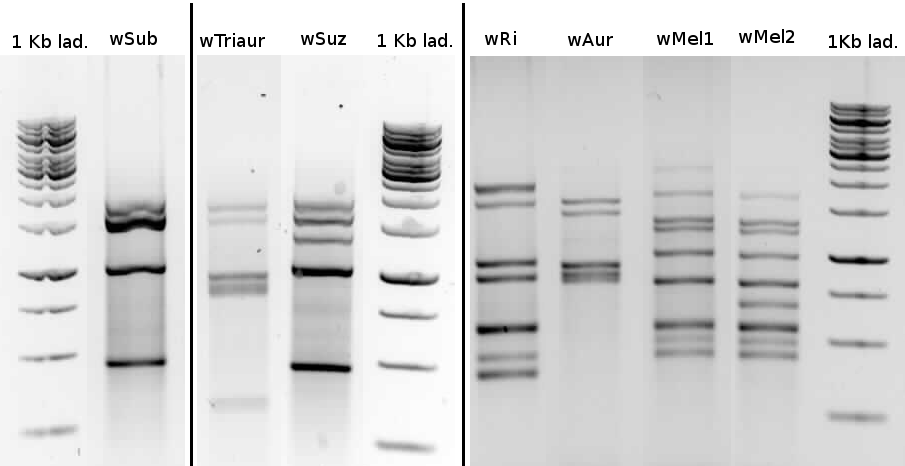
\includegraphics[width=150mm]{images/profils_crop.png}
	\end{center}
	\caption{Reconstruction d'un gel représentant tous les profils carractéristiques des souches de \esp{Wolbachia} en transposon-display avec les amorces Isb/LNP.}
	\label{fig:profils}
\end{figure}

% paragraph polymorphisme (end)



\paragraph{Une amélioration nette du protocole.} % (fold)
\label{par:proto}
Un des éléments notables dans les gels d'éléctrophorèse obtenus est la nette amélioration de l'amplification des fragments de grande taille, notamment pour les profils de type \textit{wMel} (Cf. Figure \ref{fig:wMelcomp}). 
% paragraph proto (end)
Pour les nouvelles souches passées en transposon-display, nous pouvons faire les observations suivantes : 
\begin{enumerate}
	\item \esp{wTriaur} et \esp{wAur} ont des profils similaires, ce qui peut s’expliquer par la très forte apparenté de ses hôtes.
	\item De la même façon, \esp{wSub} semble partager beaucoup fragments avec \esp{wSuz}, témoin aussi d’une forte apparenté de ses hôtes.\\
	\esp{wSuz} de son coté forme un groupe très homogène, avec un profil spécifique.
	\item Une souche de \esp{wMel} issue d’une lignée de Madagascar présente un fragment supplémentaire (wMel2 sur la figure \ref{fig:profils}).\\
	\esp{wMel} constituait jusqu’à présent un groupe très homogène.
	Un échantillonnage supplémentaire devra donc être fait dans les lignées de \esp{wMel}, notemment celles provenant de Madagascar.
	\item \esp{wRi} reste toujours un groupe bien homogène au sein de \esp{D. simulans}.
\end{enumerate}

\begin{figure}[h]
	\begin{center}
		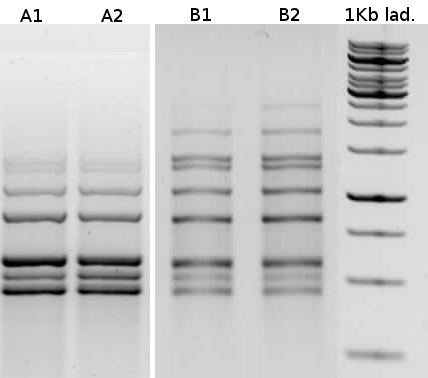
\includegraphics[width=80mm]{images/wMel_comp.png}
	\end{center}
	\caption{Comparaison des deux protocoles sur wMel (\esp{Wolbachia} de \esp{D. melanogaster})~:
	A1 et A2 : Ancien protocole\cite{memHH}~;
	B1 et B2 : Nouveau protocole, avec accuTaq}
	\label{fig:wMelcomp}
\end{figure}

% section r_sultats (end)

\section{Discussions \& Perspectives} % (fold)
\label{sec:discussions}








Afin de tirer des conclusions complètes sur les tranferts horizontaux, il faut encore attendre les résultats de transposon-display sur des lignées de \esp{L. heterotoma} infectées par une seule souche de \esp{Wolbachia}.
Nous ne possédons pas encore ces lignées, mais une seconde partie de ce stage, non développée ici; a consisté à démarrer un traitement antibiotique ménagé sur des \esp{L. heterotoma} tri-infectées (statut d'infection sauvage), afin d'obtenir des lignées présentant un statut d'infection différent pour enfin les typer en transposon-display.

La suite de ce travail consistera à séquencer les fragments obtenus afin de situer précisément les insertions dans le génome, afin d’éventuellement en tirer des conclusions sur les conséquences physiologiques des différentes insertions du transposon. Peut-être trouverons-nous là une piste pour expliquer l’adaptabilité exceptionnelle de \esp{Wolbachia} aux changements d’hôtes ?
% section conclusion_&_perspectives (end)
